\documentclass[10pt,a4paper]{article}
\usepackage[top=0in, bottom=0.5in,margin=1in, includefoot]{geometry}
\usepackage[utf8]{inputenc}
\usepackage[T1]{fontenc}
\date{}
\author{}
\setlength\parindent{0pt}
\usepackage{amsmath}
\usepackage{wrapfig}
\usepackage{graphicx}
\usepackage{lineno}
\usepackage{layout}
\setlength{\voffset}{-0.4in}
\textheight = 735pt
\begin{document}
\vspace{-20mm}
\title{\textbf{EE2-08C Numerical Analysis} \\ Group 9\vspace{-17mm}}
\maketitle
\tableofcontents
\pagebreak
\section{Exercise 3 - RLC Circuit}\vspace{-1mm}
\subsection{Background}

\begin{wrapfigure}{r}{0.5\textwidth}
\vspace{-10mm}
  		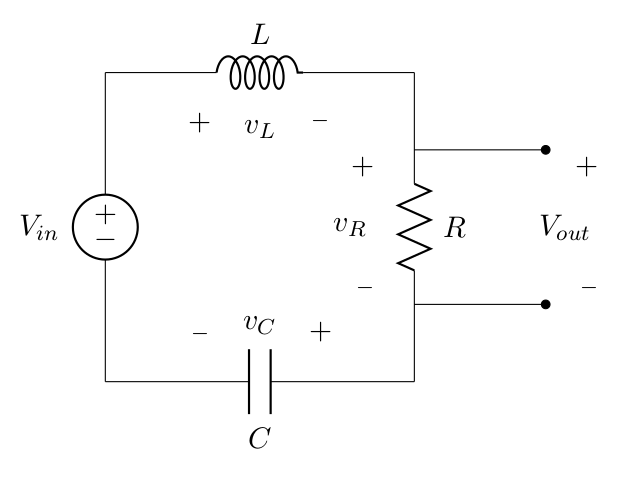
\includegraphics[width=0.49\textwidth]{Ex3_Figs/RLC.png}
\vspace{-6mm}
  	\caption{RLC Circuit}
  	\label{fig:RLC}
\end{wrapfigure}

From Kirchoff's Voltage Law (KVL) the sum of all the voltages in a closed loop must sum to 0 V. Therefore from this we can derive the equation $V_{in}(t) = v_L(t)+v_R(t)+v_C(t)$. All of the voltages in the closed loop current which flows through them, all being equal to the inductor current. The voltage across a conductor is the inductance multiplied by the derivative of it's current, the voltage across the resistor is equal to it's resistance multiplied by the current travelling through it and the voltage across the capacitor is the charge held within the capacitor divided by the capacitance of the capacitor. Substituting these characteristics into the equation above gives us the equation:

\[ L \frac{d}{dt}i_L(t) + R i_L(t) + \frac{1}{C}\int\limits_0^t i_L(t) \ dt = V_{in}(t)\]

Substituting $i_L(t)$ for $\frac{d}{dt}q_C(t)$ you make the equation:

\[ L \frac{d^2}{dt^2}q_C(t) + R\frac{d}{dt}q_C(t) + \frac{1}{C}q_C(t) = V_{in}(t)\]

We were then able to turn this second order ODE into a set of 2 coupled first order ODEs through the use of equating $q_C'(t)$ = $y(t)$ and substituting $q_C(t)$ for $x(t)$ we have the coupled equations:

\[y(t) = x'(t) \text{\hspace{5mm}and \hspace{5mm}}y'(t) = \frac{1}{L}[V_{in}(t)  - Ry(t) - \frac{1}{C}x(t)] \]

For our project we have values:

\[R = 250 \Omega, C = 3 \mu F , L = 650 mH, i_L(0) = 0 \hspace{2mm} (y_0) \text{\hspace{2mm}and\hspace{2mm}} q_C(0) = 500nC \hspace{2mm} (x_0).\]

\subsection{Script Coupled Equations and Constants}

Now that we have these two equations we are able to implement them into MATLAB scripf called `RLC\_script.m' by defining them as:

\begin{verbatim}
R = 250; L = 650*10^-3; C = 3*10^-6; %Impedance values for the components
w1 = 2*pi*500; %frequency for the 500 Hz sinusoid
w2 = 2*pi*100; %frequency for the sinusoid
w3 = 2*pi*5; %frequency for the sinusoid
tc = 3*10^-6; %tau for the exponential decay input
y0 = 0; x0 = 500*10^-9; t0 = 0; %Initial conditions y = iL, x =qC and t = time
h = 0.00001; %step size
tf = 0.03; %final condition
Vin = @(t) 5;
func1 = @(x, y, t) y; %y = q'
func2 = @(x, y, t) (Vin(t) - R*y - x/C)/L; %the second coupled equation
\end{verbatim}

\subsection{4th Order Runge Kutta 3/8 Algorithm}
\subsubsection{Theory}

To now evaluate these coupled equations, we use the Runge Kutta 4th order 3/8 algorithm to use these two coupled equations to estimate the next point of the current $i_L$ and the charge $q_C$. The algorithm is:

\[f_1(x,y,t) = y \hspace{3mm} f_2(x,y,z) = \frac{1}{L}[V_{in}(t) - Ry - \frac{x}{C}]\]
\[k1_x = hf_1(x_i,y_i,t_i) \hspace{3mm} k1_y = hf_2(x_i,y_i,t_i)\]
\[k2_x = hf_1(x_i+\frac{k1_x}{3},y_i+\frac{k1_y}{3},t_i+\frac{h}{3}) \hspace{5mm} k2_y = hf_2(x_i+\frac{k1_x}{3},y_i+\frac{k1_y}{3},t_i+\frac{h}{3})\]
\[k3_x = hf_1(x_i-\frac{k1_x}{3}+k2_x,y_i-\frac{k1_y}{3}+k2_y,t_i+\frac{2h}{3}) \]
\[k3_y = hf_2(x_i-\frac{k1_x}{3}+k2_x,y_i-\frac{k1_y}{3}+k2_y,t_i+\frac{2h}{3})\]
\[k4_x = hf_1(x_i+k1_x-k2_x+k3_x,y_ik1_y-k2_y+k3_y,t_i+h) \]
\[k4_y = hf_2(x_i+k1_x-k2_x+k3_x,y_ik1_y-k2_y+k3_y,t_i+h)\]
\[x_{i+1} =x_i+\frac{k1_x+3k2_x+3k3_x+k4_x}{8} \hspace{3mm} y_{i+1} =y_i+\frac{k1_y+3k2_y+3k3_y+k4_y}{8}\]
\[t_{i+1} = t_i + h \hspace{3mm} \text{where h is time step}\]

The way that this works is it takes several different values from around the point you are moving from and using

\subsubsection{Implementation}

To implement this into MATLAB we created a function called `RK4second.m' in which would take in the two functions and work out the k efficients for both x and y and from there, work out the next position of the x (charge) and y (current) coordinates.

\begin{verbatim}
function [xout, yout] = RK4second (xin, yin, h, tin, func1, func2)

	k1x = h*feval(func1, xin ,yin, tin); %approx the first consts for RK4th ord 3/8 Method
k1y = h*feval(func2, xin ,yin, tin);
	k2x = h*feval(func1, xin + k1x/3, yin + k1y/3, tin+h/3);
	k2y = h*feval(func2, xin + k1x/3, yin + k1y/3, tin+h/3);
	k3x = h*feval(func1, xin  - k1x/3 + k2x, yin - k1y/3 + k2y, tin+2*h/3);
	k3y = h*feval(func2, xin  - k1x/3 + k2x, yin - k1y/3 + k2y, tin+2*h/3);
	k4x = h*feval(func1, xin + k1x - k2x + k3x, yin + k1y - k2y + k3y, tin+h);
k4y = h*feval(func2, xin + k1x - k2x + k3x, yin + k1y - k2y + k3y, tin+h);

	xout = xin + (k1x + 3*k2x + 3*k3x + k4x)/8;
	yout = yin + (k1y + 3*k2y + 3*k3y + k4y)/8;
end
\end{verbatim}

This takes in the present value of current and charge a certain time, the time position, the step time and the two functions to evaluate and approximate the next point, which is then outputted at the end.

\subsection{RLC\_Script.m Implementation}

\begin{verbatim}
N = round((tf-t0)/h); %calculates number of time steps
ya = zeros(1,N); xa = zeros(1,N);
ta = zeros(1,N); in = zeros(1,N); %set up arrays

xa(1) = x0; ya(1) = y0; ta(1) = t0; in(1) = Vin(t0); %input initial conditions
for i = 1:N-1 %works out next timestep value
	   [xa(i+1), ya(i+1)] = RK4second (xa(i), ya(i), h, ta(i),func1, func2);
    ta(i+1) = ta(i) + h; %next time step
    in(i+1) = Vin(ta(i+1)); %next value of the input
end

figure; %sets up the figures
Vout = R*ya; %Vout = R*iL
subplot(2,1,1);
plot(ta, Vout); %plot output Voltage
grid on;
xlabel('Time/s'); ylabel('Voltage Out/V');
title('R*dq/dt with a Step Response')
subplot(2,1,2);
plot(ta, in); %plot input Voltage
grid on;
xlabel('Time/s'); ylabel('Voltage In/V');
title('Step Response')
\end{verbatim}

\pagebreak

\subsection{Exercise 3 Graphs}
\subsubsection{Step Response}

\begin{wrapfigure}[13]{r}{0.5\textwidth}

	\vspace{-6mm}
  		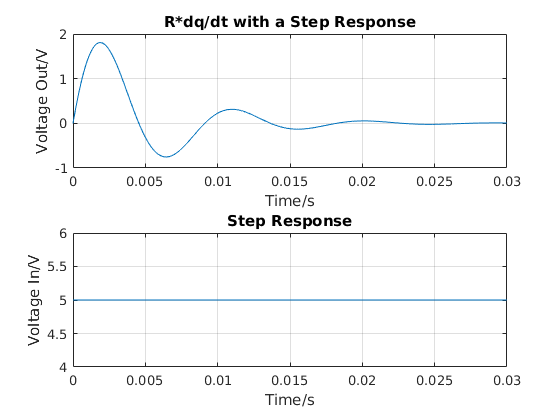
\includegraphics[width=0.49\textwidth]{Ex3_Figs/Step.png}
	\vspace{-6mm}
  	\caption{$V_{in}(t)= 5$}
  	\label{fig:ex3g1}

\end{wrapfigure}

    \vspace{0mm}The step response causes a sudden rise of voltage up to 5 V, due to the inductor not being able to change current instantaneously the voltage out starts from 0 V and as you can see on Figure 2. It increases up to around 1.8 V at this point the capacitor starts to reduce the rate of it charging up due to saturating in charge, as the voltage out starts to tend to 0, the capacitor emits charge causing a negative current through the inductor. As this goes on, the voltage across the capacitor tends to 5 V causing no current to flow through the inductor and the resistor, causing the output voltage to tend to 0 V.

\subsubsection{Sine Wave Input}

\begin{wrapfigure}[13]{r!}{0.5\textwidth}
    \vspace{-7mm}

  		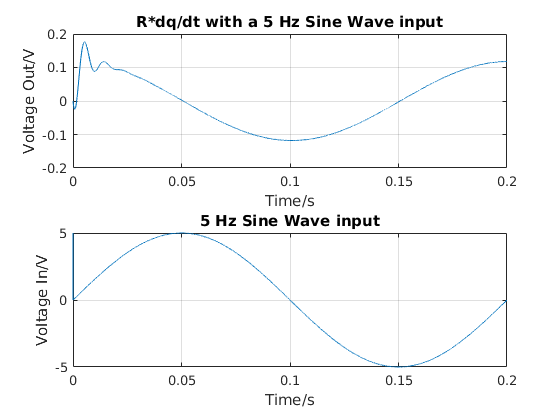
\includegraphics[width=0.49\textwidth]{Ex3_Figs/5Sine2.png}
	\vspace{-6mm}
  	\caption{$V_{in}(t)= 5sin(2 \pi 5t)$}
  	\label{fig:ex3g2}

\end{wrapfigure}

\vspace{0mm}In Figure 3 the input is a sine wave of amplitude 5 V and a frequency of 5 Hz, as the sine wave moves away from zero it causes a sharp increase in the current going through the inductor and therefore causes a sharp rise on the voltage out, this then attenuates to form the shape of a sine wave of amplitude is $\approx 0.1$ V and leads the input voltage by a phase difference of $\frac{\pi}{2}$ this is relative to the frequency of the input and the complex impedance of both the inductor and the capacitor being $j\omega L$ and $\frac{1}{j\omega C}$ respectively. We chose the final time as 0.2 s to show how initially the output changes but then follows the shape of the input eventually.

\begin{wrapfigure}[16]{r}{0.5\textwidth}
    \vspace{-5mm}
  		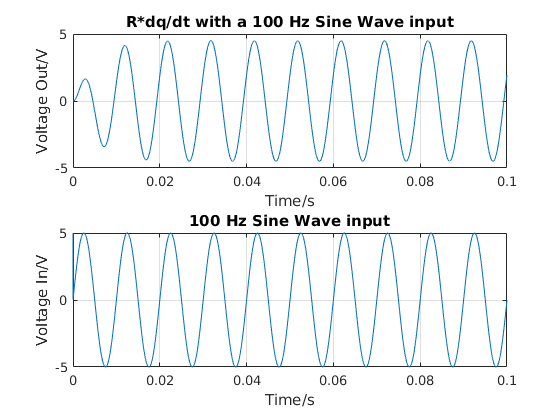
\includegraphics[width=0.48\textwidth]{Ex3_Figs/100Sine.png}
	\vspace{-6mm}
  	\caption{$V_{in}(t)= 5sin(2 \pi 100t)$}
  	\label{fig:ex3g3}
\end{wrapfigure}
\vspace{6mm}In Figure 4 the input is a sine wave of amplitude 5 V and a frequency of 100 Hz. Upon the start of the wave, the output voltage rises slower than the voltage of the input, due to the fact that the rate of change of the inductor current cannot shange instantaneously and will eventually equal the frequency of the input. This causes a slight phase difference and the amplitude is far greater than the 5 Hz input, resulting in an amplitude of $\approx 4$ V. This greater output voltage is due to being a band pass filter, low frequencies as we can see, 5 Hz for example attenuate to a value close to 0 V whereas at this frequency the output voltage is close to the input voltage and at some frequency greater than this, the same result as the 5 Hz wave will be apparent.

\begin{wrapfigure}[11]{r}{0.5\textwidth}
    \vspace{-12mm}
  		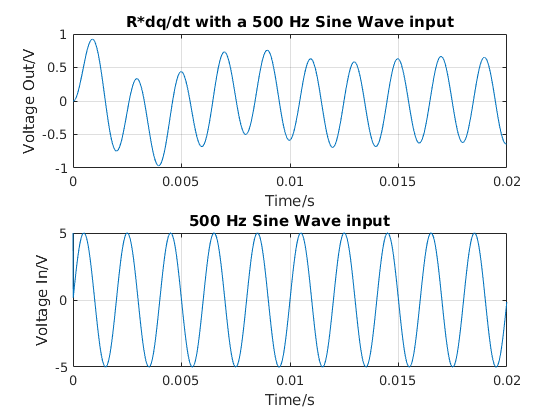
\includegraphics[width=0.48\textwidth]{Ex3_Figs/500Sine.png}
	\vspace{-6mm}
  	\caption{$V_{in}(t)= 5sin(2 \pi 500t)$}
  	\label{fig:ex3g4}
\end{wrapfigure}

\vspace{2mm}In Figure 5 the input is a sine wave of amplitude 5 V and a frequency of 500 Hz. The response is very similar to Figure 3's output signal, rising initially to a value that is greater than its steady state amplitude in which is $\approx 0.5$ V which is far 10 times less than the input amplitude, and less than the the amplitude of the Figure 4. This suggests that the center of the band pass filter is based around 100 Hz as is seen in Figure 4 and therefore the outer bounds falling in amplitude at frequencies greater and less than this.

\pagebreak
\subsubsection{Square Wave Inputs}

\begin{wrapfigure}[11]{r}{0.5\textwidth}
    \vspace{-7mm}
  		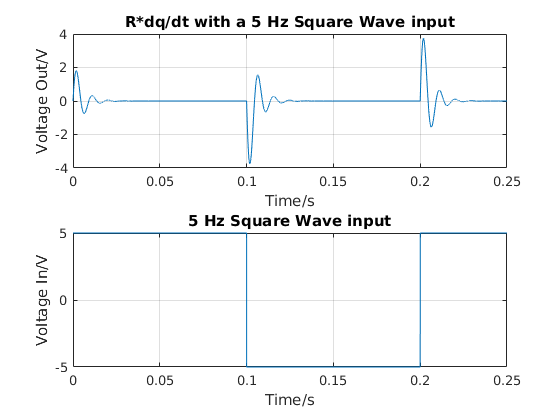
\includegraphics[width=0.48\textwidth]{Ex3_Figs/5Squ1.png}
	\vspace{-6mm}
  	\caption{$V_{in}(t)= 5square(2 \pi 5t)$}
  	\label{fig:ex3g5}
\end{wrapfigure}

\vspace{3mm}In Figure 6 the input is a square wave of frequency 5 Hz and amplitude 5 V. At this frequency, the response is identical to the response of a step response due to there being enough time for the wave to return to 0 V after the change in amplitude, the only difference is when the voltage drops to -5 V the step response is equal to the positive step response but negative. The time scale was chosen to show 1 and a quarter wavelengths so that it is easy to see that each time the sign changes, the response is identical.

\begin{wrapfigure}[8]{r}{0.5\textwidth}
    \vspace{-6mm}
  		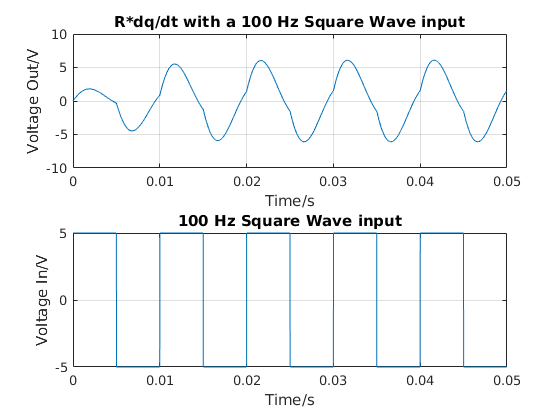
\includegraphics[width=0.48\textwidth]{Ex3_Figs/100Squ1.png}
	\vspace{-6mm}
  	\caption{$V_{in}(t)= 5square(2 \pi 100t)$}
  	\label{fig:ex3g6}
\end{wrapfigure}

\vspace{15mm}In Figure 7 the input is a square wave of frequency 100 Hz and amplitude 5 V. At this frequency, the output follows the characteristic of a sine wave due to the step response giving a sinusoidal peak, this is repeated but switched in direction as the sign of the input changes, causing a periodic signal on the output respresenting something somewhat similar to a sine wave.

\begin{wrapfigure}[17]{r}{0.5\textwidth}
    \vspace{7mm}
  		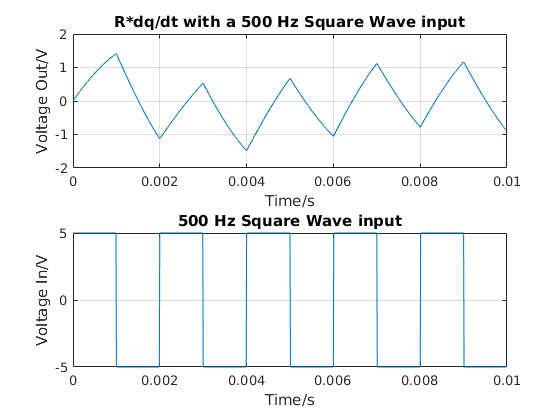
\includegraphics[width=0.48\textwidth]{Ex3_Figs/500Squ1.png}
	\vspace{-6mm}
  	\caption{$V_{in}(t)= 5square(2 \pi 500t)$}
  	\label{fig:ex3g7}
\end{wrapfigure}

\vspace{14mm}In Figure 8, the input is a square wave of frequency 500 Hz and amplitude 5 V. At this frequency, the step responses cause an output signal which is similar to a periodic tent function of exponential charge and discharge, this is due to the fact that the square wave changes sign too rapidly for the signal to smooth off or return to zero before the next half wavelength. As it gets to the 4th period of the input, the output settles to an amplitude of $\approx 1$ V. In which looking back over Figures 6, 7 and 8. The bandpass filter seems to give similar changes in output amplitude relative to the input amplitude, where at 100 Hz, in Figure 7 the magnitude is greater than both magnitudes. Confirming that the center frequency if based around 100 Hz and the bandwidth is based between 5 Hz and 500 Hz.

\subsubsection{Exponential Decay Input}

\begin{wrapfigure}[9]{r}{0.5\textwidth}
    \vspace{-7mm}
  		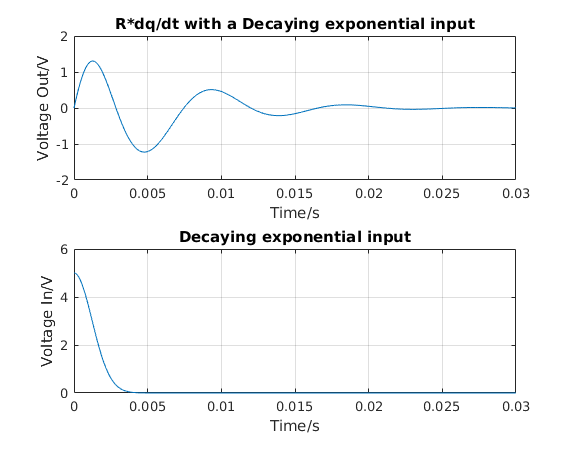
\includegraphics[width=0.48\textwidth]{Ex3_Figs/DecExp.png}
	\vspace{-6mm}
  	\caption{$V_{in}(t)= 5e^{\frac{-t^2}{\tau_C}}$}
  	\label{fig:ex3g8}
\end{wrapfigure}

In Figure 9, the input is a decaying exponential in which it's time constant $\tau_C = 3 (ms)^2$ causing a sharp drop in amplitude towards 0 V in a time of less than 5 ms, causing an output in which is incredibly similar to the output of the step responss (Figure 2). The only main difference being that the max amplitude of the output of Figure 9 is $\approx 1$ V, $\approx 0.8$ V less than the max amplitude of Figure 2 in which the amplitude was $\approx 1.8$ V.

\pagebreak

\section{Exercise 4 - Finite Differences for PDE}\vspace{-1mm}
\subsection{Background}

For this exercise we were asked to implement the finite difference method for the 1D heat equation which is:

\[\frac{\partial y}{\partial t} = \frac{\partial^2 x}{\partial t^2}\ \hspace{5mm} \text{in which} \hspace{5mm} 0 < x < 1, \hspace{5mm} t > 0 \hspace{5mm} \text{and} \hspace{5mm} y(0,t) = y(1,t) = 0 \hspace{2mm} \forall \hspace{2mm} t\]

\begin{verbatim}
x0 = 0;
h = 0.005; %Step size in the X direction
Vin = @(x) sin(2*pi*x);
Bc = @(t) 0;
xf = 1 + h; %Final value of X untitledplus one more step to complete the graph
t0 = 0; %Initial time value
k = 0.45*h^2; %v max of 1/2 we use 0.45 work out k relatively, steps in time
tf = 200*k; %the end time is 250 steps in the k direction
N = round((xf-x0)/h); %number of steps in the x direction
M = round((tf - t0)/k); %number of steps in the t direction
v = k/(h^2); %recalculating the value of v
b = 1 - 2*v; %create the value of beta
ya = zeros(1,N); xa = zeros(1,N); %create empty arrays
xa(1) = x0; xa(N) = xf-h;  ya(1) = Bc(0); ya(N) = Bc(0); %initial conditions
\end{verbatim}

\end{document}
